%CS51 HW9 Assignment
%Preamble
\documentclass[12pt, letterpaper]{article}
\usepackage[utf8]{inputenc}
\usepackage{graphicx}
\usepackage{comment}
\usepackage{subcaption}
\usepackage[export]{adjustbox}
\usepackage[margin=0.25in]{geometry}
\graphicspath{
{/Users/carterbastian/Desktop/dgood/}{/Users/carterbastian/Desktop/dbad/} }

\usepackage{cleveref}


\title{Data Hazard Demonstration}
\author{Carter J. Bastian \thanks{COSC51 HW9 Q4}}
\date{May 2015}

\begin{document}
\maketitle
% Figure 1 = Step 1 (d1)
\begin{figure}[h]
  % dgood1
  \begin{subfigure}{0.5\textwidth}
    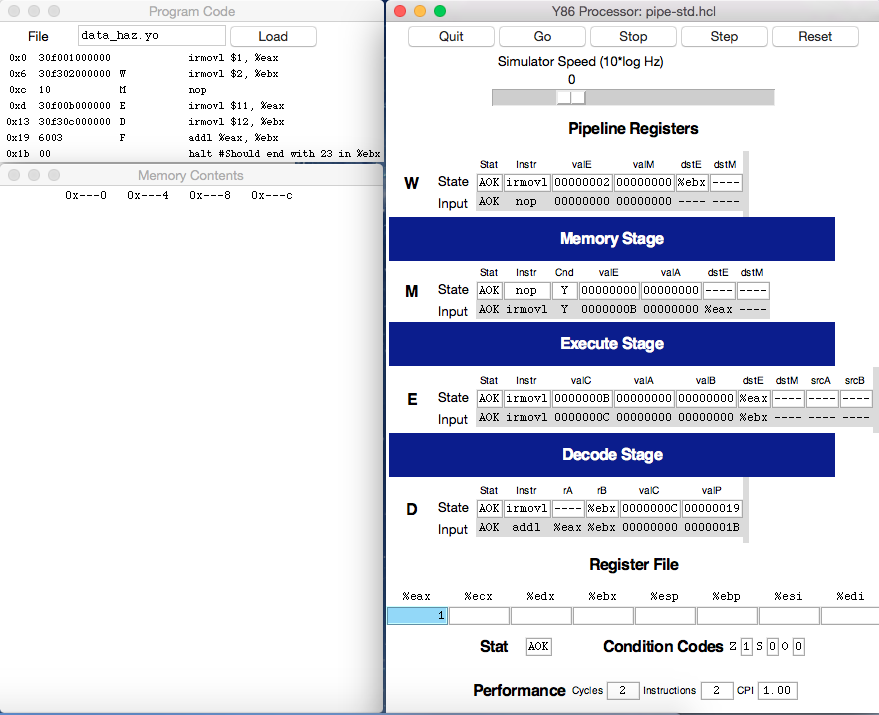
\includegraphics[scale=.33]{dgood1}
    \caption{Correct Implementation (std)}
    \label{fig:dgood1}
    \end{subfigure}
  % dbad1
  \begin{subfigure}{0.5\textwidth}
    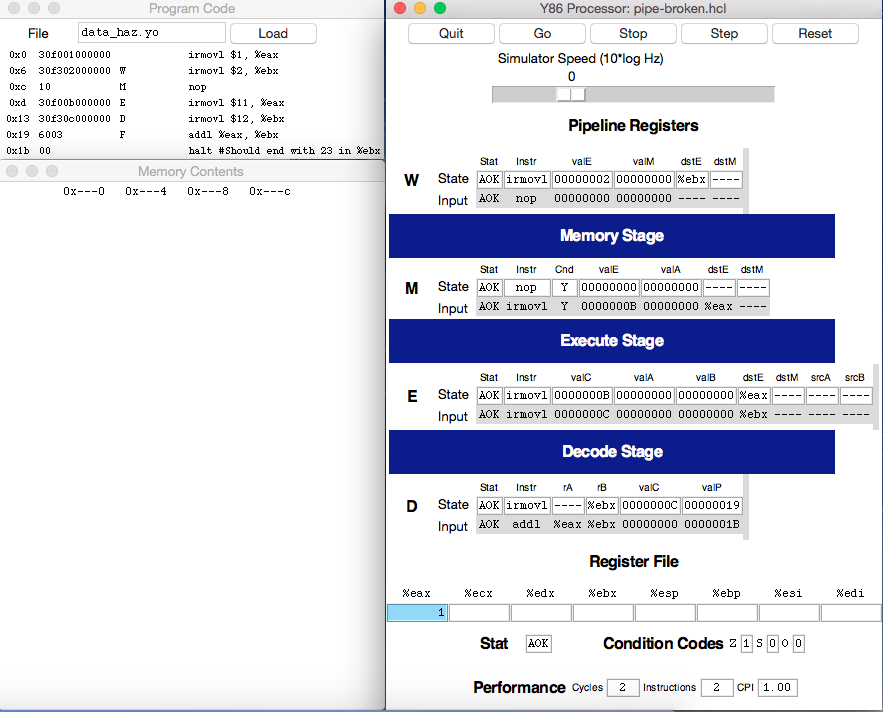
\includegraphics[scale=.33, right]{dbad1}
    \caption{Incorrect Implementation (broken)}
    \label{fig:dbad1}
  \end{subfigure}
  \caption{In this step, the \texttt{addl \%eax, \%ebx} instruction has just been
fetched by the two different versions. Note that there are two
irmovl instructions writing to registers \texttt{\%eax} and \texttt{\%ebx} in
the Execute and Decode Pipeline Registers respectively.}
  \label{fig:d1}
\end{figure}
% Figure 2 = Step 2 (d2)
\begin{figure}[h]
  % dgood2
  \begin{subfigure}{0.5\textwidth}
    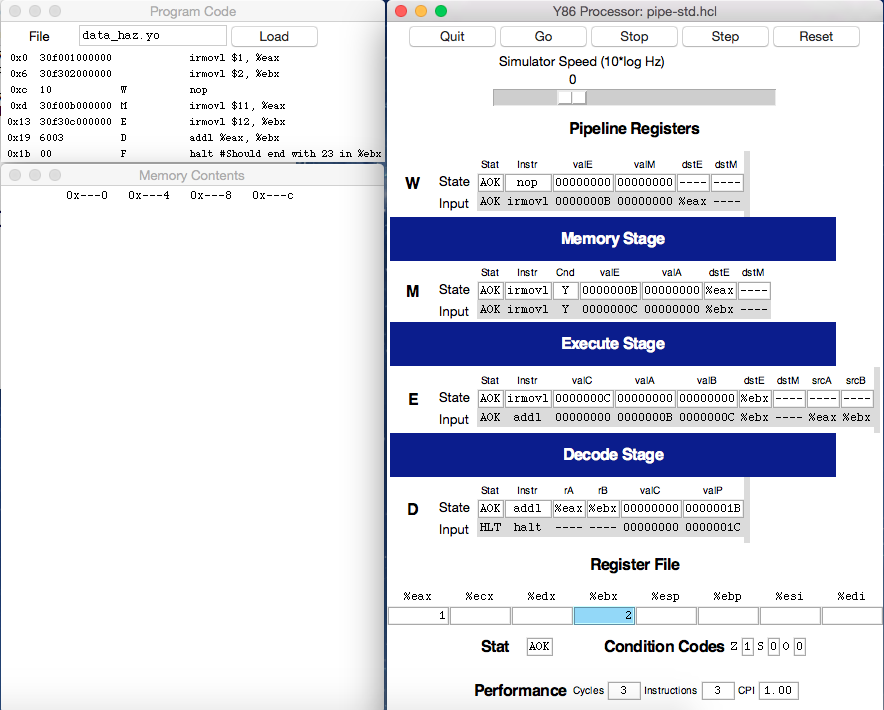
\includegraphics[scale=.33]{dgood2}
    \caption{Correct Implementation (std)}
    \label{fig:dgood2}
    \end{subfigure}
  % dbad2
  \begin{subfigure}{0.5\textwidth}
    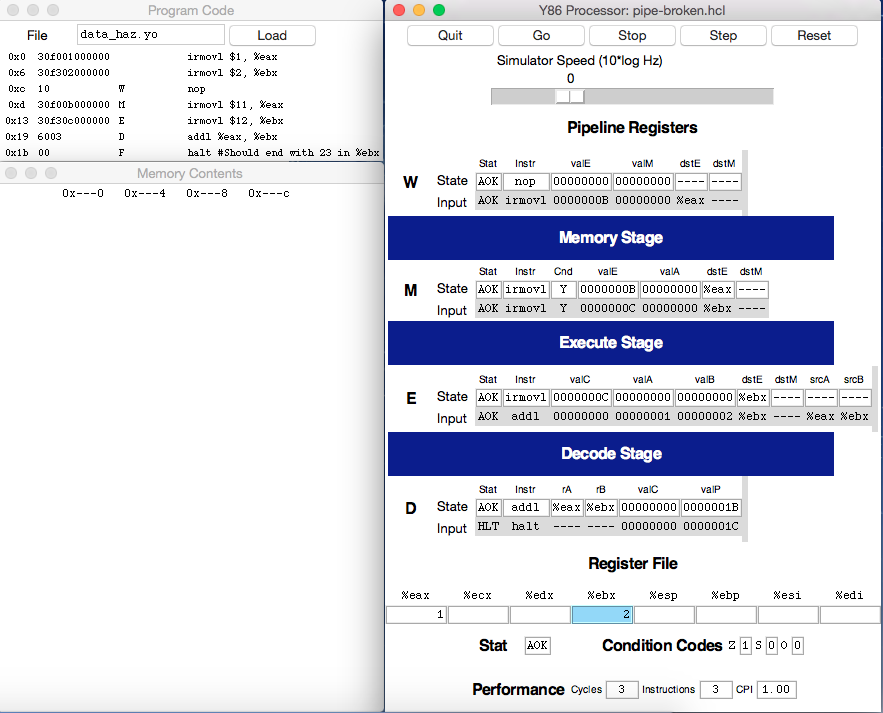
\includegraphics[scale=.33, right]{dbad2}
    \caption{Incorrect Implemenetation (broken)}
    \label{fig:dbad2}
  \end{subfigure}
  \caption{In this step, both implementations' programmer-visible states are
still identical as the \emph{addl} instruction is moved into the Decode Pipeline
Register.}
  \label{fig:d2}
\end{figure}
% Figure 3 = Step 3 (d1)
\begin{figure}[h]
  % dgood3
  \begin{subfigure}{0.5\textwidth}
    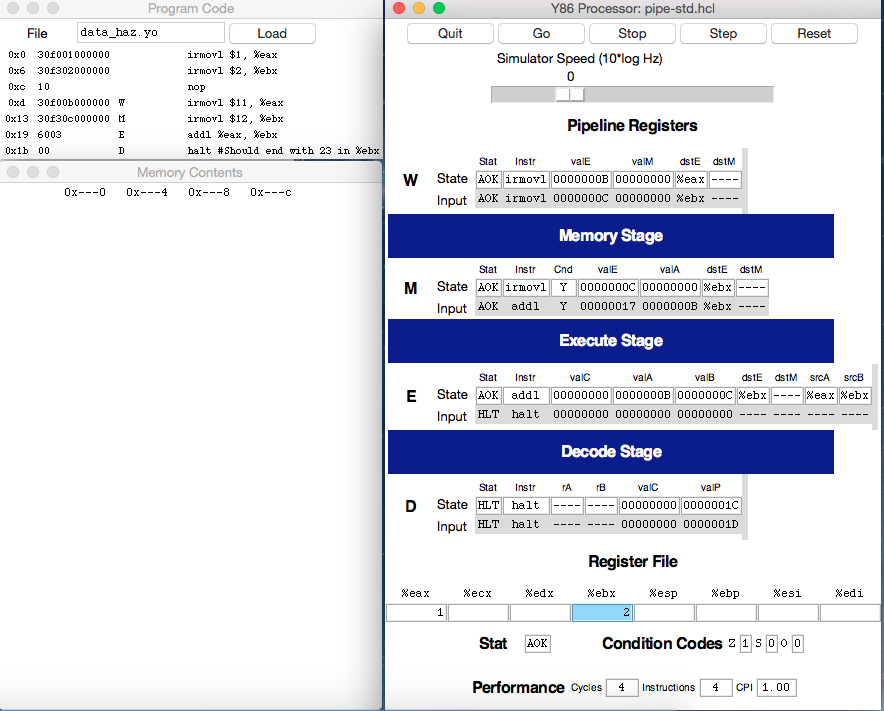
\includegraphics[scale=.33]{dgood3}
    \caption{Correct Implementation (std)}
    \label{fig:dgood3}
    \end{subfigure}
  % dbad3
  \begin{subfigure}{0.5\textwidth}
    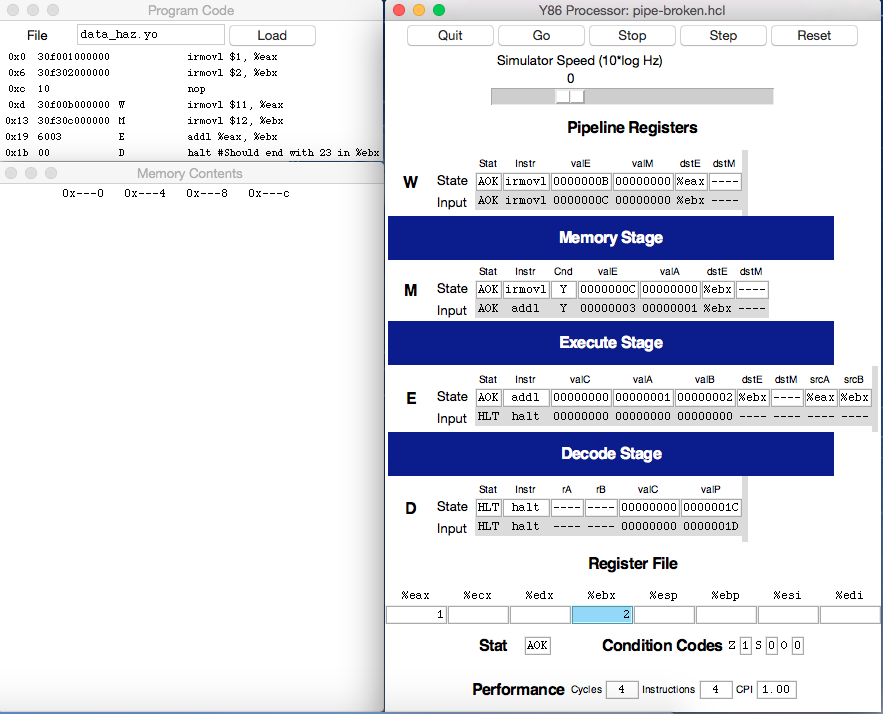
\includegraphics[scale=.33, right]{dbad3}
    \caption{Incorrect Implementation (broken)}
    \label{fig:dbad3}
  \end{subfigure}
  \caption
{Here we can clearly see where the data hazard arises. When the correct
implementation decoded \texttt{rA} and \texttt{rB}, it forwarded the values
still in the process of being written by the two \texttt{irmovl} instructions
still in the Write and Memory Pipeline Registers. \\ In contrast, the incorrect
implementation decoded \texttt{rA} and \texttt{rB} to be the values written by
the \texttt{irmovl} instructions from lines 1 and 2 (which have already been
written). As a result, there's a disparity between the \texttt{valA} and
\texttt{valB} values in the Execute Pipeline Registers of the two
implementations. The incorrect version is using outdated values as its operands.}
  \label{fig:d3}
\end{figure}
% Figure 4 = Step 4 (d4)
\begin{figure}[h]
  % dgood4
  \begin{subfigure}{0.5\textwidth}
    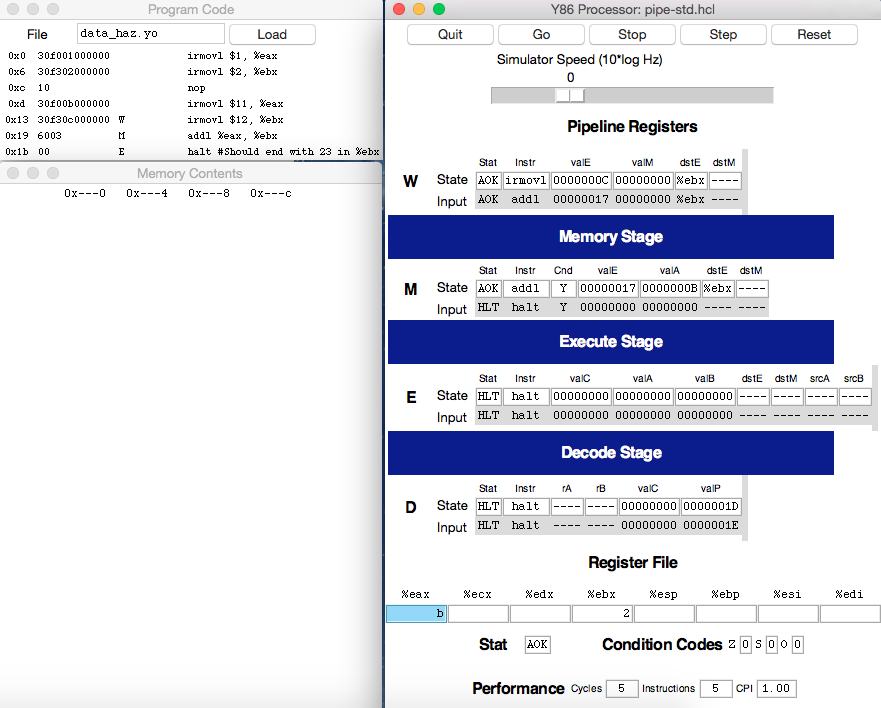
\includegraphics[scale=.33]{dgood4}
    \caption{Correct Implementation (std)}
    \label{fig:dgood4}
    \end{subfigure}
  % dbad4
  \begin{subfigure}{0.5\textwidth}
    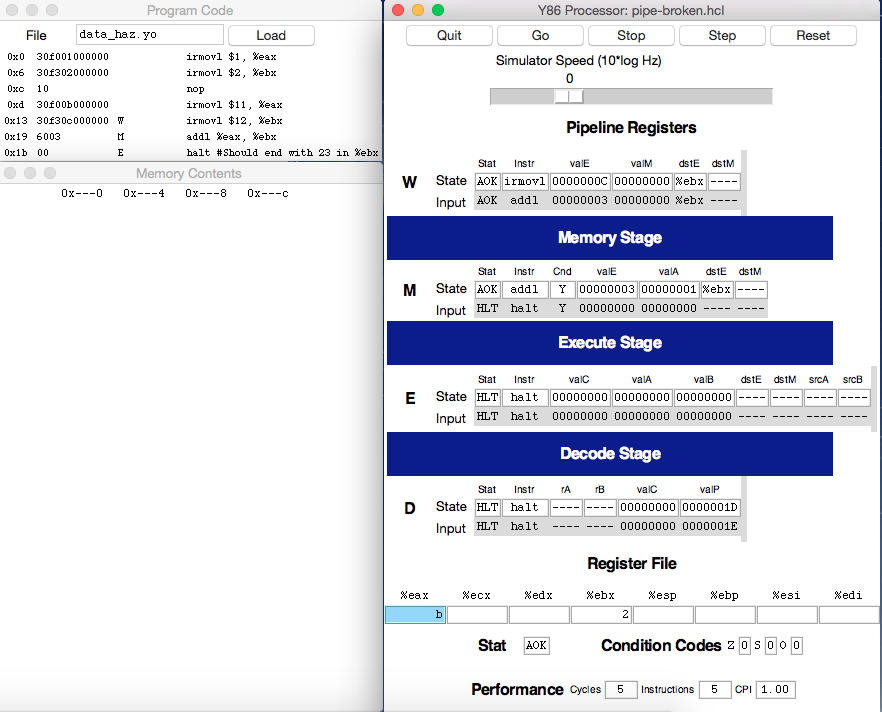
\includegraphics[scale=.33, right]{dbad4}
    \caption{Incorrect Implementation (broken)}
    \label{fig:dbad4}
  \end{subfigure}
  \caption
{In this state, the \texttt{irmovl} instruction writing to register
\texttt{\%eax} goes the the write-back stage. The \texttt{addl} instruction
moves into the Memory Pipeline Register. Notice the correct value of the sum is
in Figure (\subref{fig:dgood4}) \texttt{valE}, while an incorrect value of the
sum is in Figure (\subref{fig:dbad4}) \texttt{valE}. }
  \label{fig:d4}
\end{figure}
% Figure 5 = Step 5 (d5)
\begin{figure}[h]
  % dgood5
  \begin{subfigure}{0.5\textwidth}
    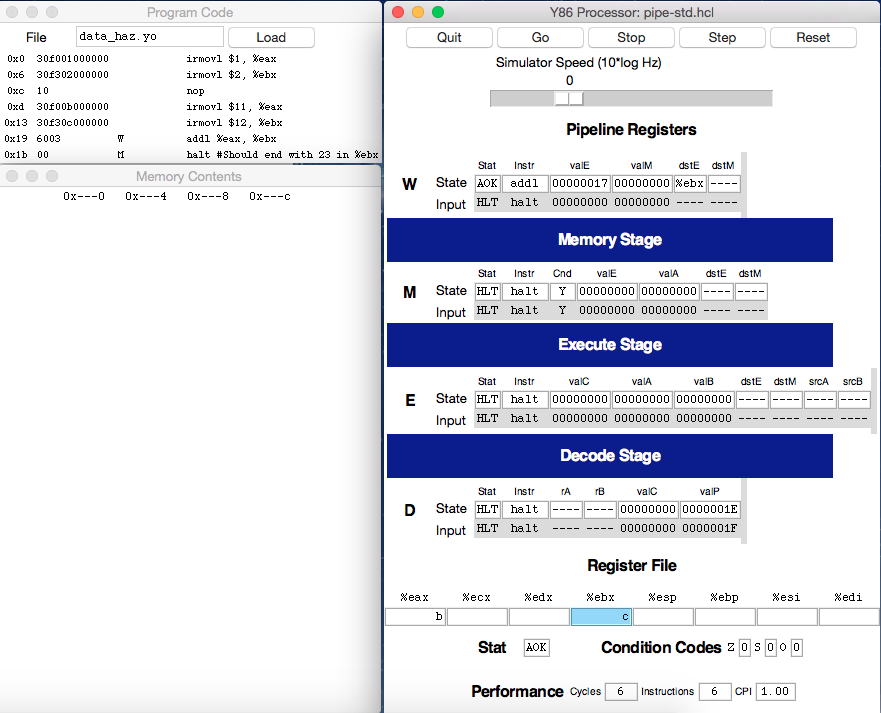
\includegraphics[scale=.33]{dgood5}
    \caption{Correct Implementation (std)}
    \label{fig:dgood5}
    \end{subfigure}
  % dbad5
  \begin{subfigure}{0.5\textwidth}
    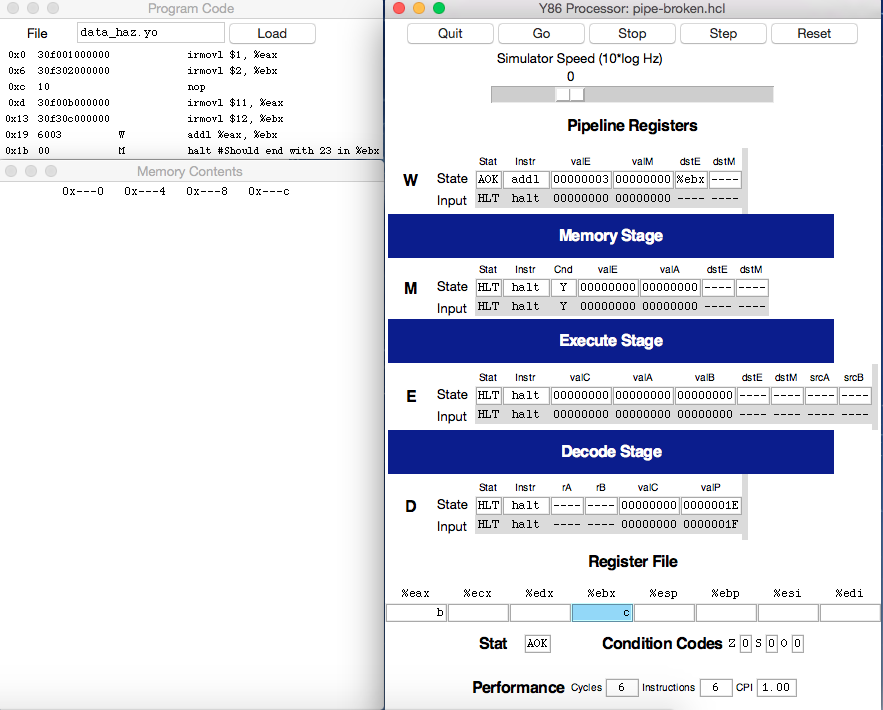
\includegraphics[scale=.33, right]{dbad5}
    \caption{Incorrect Implementation (broken)}
    \label{fig:dbad5}
  \end{subfigure}
  \caption{The \texttt{addl} instruction moves into the Write Pipeline
Register.}
  \label{fig:d5}
\end{figure}
% Figure 6 = Step 6 (d6)
\begin{figure}[h]
  % dgood6
  \begin{subfigure}{0.5\textwidth}
    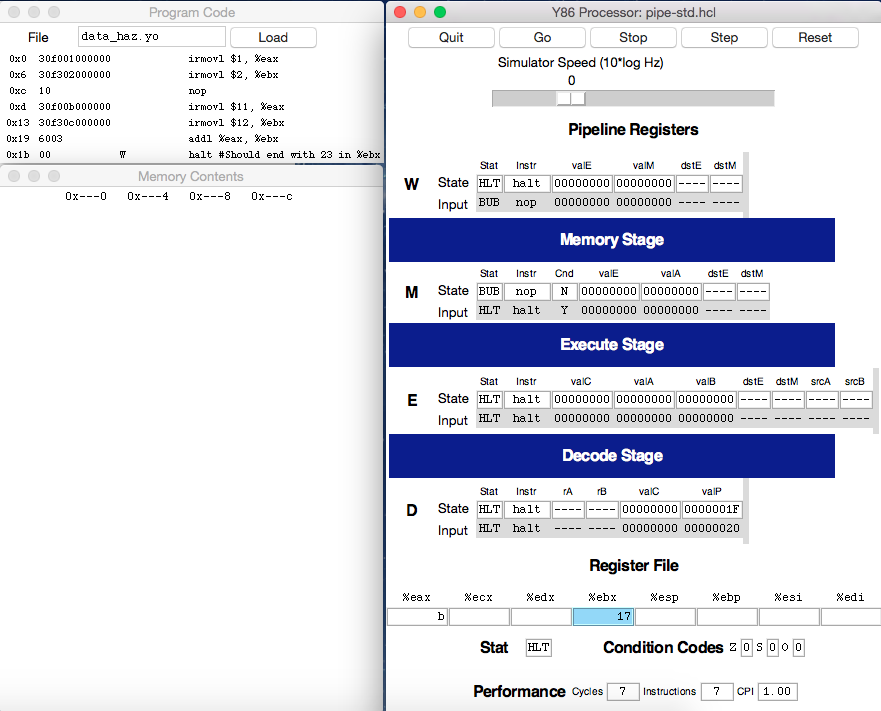
\includegraphics[scale=.33]{dgood6}
    \caption{Correct Implementation (std)}
    \label{fig:dgood6}
    \end{subfigure}
  % dbad6
  \begin{subfigure}{0.5\textwidth}
    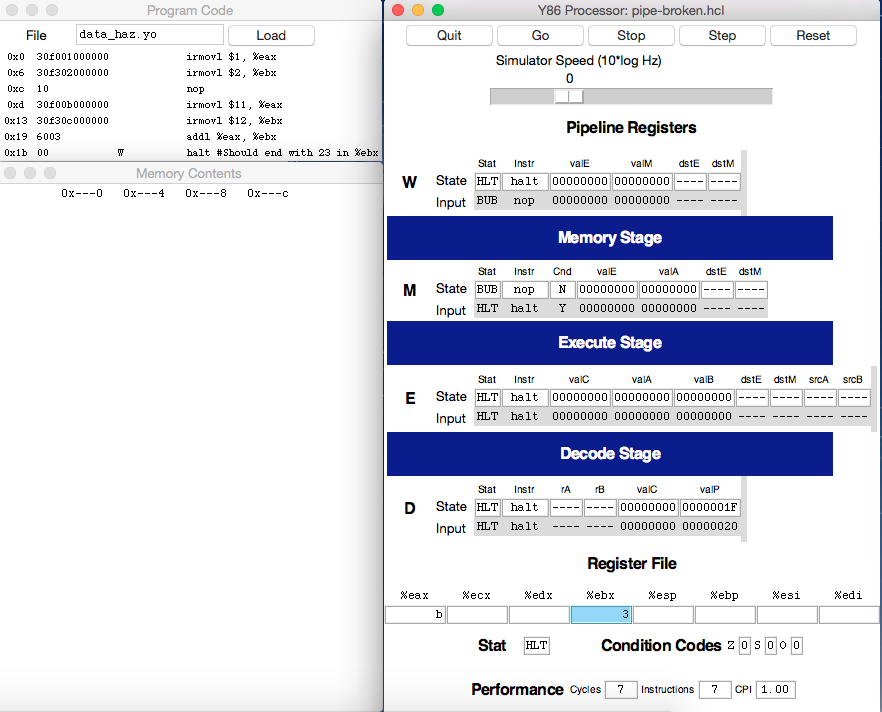
\includegraphics[scale=.33, right]{dbad6}
    \caption{Incorrect Implementation (broken)}
    \label{fig:dbad6}
  \end{subfigure}
  \caption{The sum calculated in the \texttt{addl} instruction is written back
to register \texttt{\%eax}. As you can see, due to the data hazard, the correct
sum of $11 + 12 = 23$ (in hex, \texttt{0x17}) is calculated by the correct
pipelining implementation and written to register \texttt{\%eax} in Figure 
(\subref{fig:dgood6}). \\ On the other hand, you can see the incorrect sum of $1 +
2 = 3$ is calculated by the incorrect pipelining implementation and is written
to register \texttt{\%eax} in Figure (\subref{fig:dbad6}). This displays a data
hazard.}
  \label{fig:d6}
\end{figure}
\end{document}
